\documentclass[twoside]{book}

% Packages required by doxygen
\usepackage{calc}
\usepackage{doxygen}
\usepackage{graphicx}
\usepackage[utf8]{inputenc}
\usepackage{makeidx}
\usepackage{multicol}
\usepackage{multirow}
\usepackage{fixltx2e}
\PassOptionsToPackage{warn}{textcomp}
\usepackage{textcomp}
\usepackage[nointegrals]{wasysym}
\usepackage[table]{xcolor}

% Font selection
\usepackage[T1]{fontenc}
\usepackage{mathptmx}
\usepackage[scaled=.90]{helvet}
\usepackage{courier}
\usepackage{amssymb}
\usepackage{sectsty}
\renewcommand{\familydefault}{\sfdefault}
\allsectionsfont{%
  \fontseries{bc}\selectfont%
  \color{darkgray}%
}
\renewcommand{\DoxyLabelFont}{%
  \fontseries{bc}\selectfont%
  \color{darkgray}%
}
\newcommand{\+}{\discretionary{\mbox{\scriptsize$\hookleftarrow$}}{}{}}

% Page & text layout
\usepackage{geometry}
\geometry{%
  a4paper,%
  top=2.5cm,%
  bottom=2.5cm,%
  left=2.5cm,%
  right=2.5cm%
}
\tolerance=750
\hfuzz=15pt
\hbadness=750
\setlength{\emergencystretch}{15pt}
\setlength{\parindent}{0cm}
\setlength{\parskip}{0.2cm}
\makeatletter
\renewcommand{\paragraph}{%
  \@startsection{paragraph}{4}{0ex}{-1.0ex}{1.0ex}{%
    \normalfont\normalsize\bfseries\SS@parafont%
  }%
}
\renewcommand{\subparagraph}{%
  \@startsection{subparagraph}{5}{0ex}{-1.0ex}{1.0ex}{%
    \normalfont\normalsize\bfseries\SS@subparafont%
  }%
}
\makeatother

% Headers & footers
\usepackage{fancyhdr}
\pagestyle{fancyplain}
\fancyhead[LE]{\fancyplain{}{\bfseries\thepage}}
\fancyhead[CE]{\fancyplain{}{}}
\fancyhead[RE]{\fancyplain{}{\bfseries\leftmark}}
\fancyhead[LO]{\fancyplain{}{\bfseries\rightmark}}
\fancyhead[CO]{\fancyplain{}{}}
\fancyhead[RO]{\fancyplain{}{\bfseries\thepage}}
\fancyfoot[LE]{\fancyplain{}{}}
\fancyfoot[CE]{\fancyplain{}{}}
\fancyfoot[RE]{\fancyplain{}{\bfseries\scriptsize Generated on Thu May 15 2014 10\+:21\+:19 for M\+T\+Random by Doxygen }}
\fancyfoot[LO]{\fancyplain{}{\bfseries\scriptsize Generated on Thu May 15 2014 10\+:21\+:19 for M\+T\+Random by Doxygen }}
\fancyfoot[CO]{\fancyplain{}{}}
\fancyfoot[RO]{\fancyplain{}{}}
\renewcommand{\footrulewidth}{0.4pt}
\renewcommand{\chaptermark}[1]{%
  \markboth{#1}{}%
}
\renewcommand{\sectionmark}[1]{%
  \markright{\thesection\ #1}%
}

% Indices & bibliography
\usepackage{natbib}
\usepackage[titles]{tocloft}
\setcounter{tocdepth}{3}
\setcounter{secnumdepth}{5}
\makeindex

% Hyperlinks (required, but should be loaded last)
\usepackage{ifpdf}
\ifpdf
  \usepackage[pdftex,pagebackref=true]{hyperref}
\else
  \usepackage[ps2pdf,pagebackref=true]{hyperref}
\fi
\hypersetup{%
  colorlinks=true,%
  linkcolor=blue,%
  citecolor=blue,%
  unicode%
}

% Custom commands
\newcommand{\clearemptydoublepage}{%
  \newpage{\pagestyle{empty}\cleardoublepage}%
}


%===== C O N T E N T S =====

\begin{document}

% Titlepage & ToC
\hypersetup{pageanchor=false,
             bookmarks=true,
             bookmarksnumbered=true,
             pdfencoding=unicode
            }
\pagenumbering{roman}
\begin{titlepage}
\vspace*{7cm}
\begin{center}%
{\Large M\+T\+Random }\\
\vspace*{1cm}
{\large Generated by Doxygen 1.8.7}\\
\vspace*{0.5cm}
{\small Thu May 15 2014 10:21:19}\\
\end{center}
\end{titlepage}
\clearemptydoublepage
\tableofcontents
\clearemptydoublepage
\pagenumbering{arabic}
\hypersetup{pageanchor=true}

%--- Begin generated contents ---
\chapter{Namespace Index}
\section{Namespace List}
Here is a list of all documented namespaces with brief descriptions\+:\begin{DoxyCompactList}
\item\contentsline{section}{\hyperlink{namespace_u_m_t}{U\+M\+T} }{\pageref{namespace_u_m_t}}{}
\end{DoxyCompactList}

\chapter{Hierarchical Index}
\section{Class Hierarchy}
This inheritance list is sorted roughly, but not completely, alphabetically\+:\begin{DoxyCompactList}
\item \contentsline{section}{M\+T\+Random}{\pageref{class_m_t_random}}{}
\item Random\begin{DoxyCompactList}
\item \contentsline{section}{U\+M\+T.\+Mersenne\+Twister}{\pageref{class_u_m_t_1_1_mersenne_twister}}{}
\end{DoxyCompactList}
\item \contentsline{section}{U\+M\+T.\+Wave\+To\+Rgb}{\pageref{class_u_m_t_1_1_wave_to_rgb}}{}
\end{DoxyCompactList}

\chapter{Class Index}
\section{Class List}
Here are the classes, structs, unions and interfaces with brief descriptions\+:\begin{DoxyCompactList}
\item\contentsline{section}{\hyperlink{class_u_m_t_1_1_mersenne_twister}{U\+M\+T.\+Mersenne\+Twister} \\*Generates pseudo-\/random numbers using the Mersenne Twister algorithm. }{\pageref{class_u_m_t_1_1_mersenne_twister}}{}
\item\contentsline{section}{\hyperlink{class_m_t_random}{M\+T\+Random} \\*M\+T random interface. }{\pageref{class_m_t_random}}{}
\item\contentsline{section}{\hyperlink{class_u_m_t_1_1_wave_to_rgb}{U\+M\+T.\+Wave\+To\+Rgb} }{\pageref{class_u_m_t_1_1_wave_to_rgb}}{}
\end{DoxyCompactList}

\chapter{Namespace Documentation}
\hypertarget{namespace_u_m_t}{\section{Package U\+M\+T}
\label{namespace_u_m_t}\index{U\+M\+T@{U\+M\+T}}
}
\subsection*{Classes}
\begin{DoxyCompactItemize}
\item 
class {\bfseries Exponential\+Distribution}
\item 
class {\bfseries Gamma\+Distribution}
\item 
class \hyperlink{class_u_m_t_1_1_mersenne_twister}{Mersenne\+Twister}
\begin{DoxyCompactList}\small\item\em Generates pseudo-\/random numbers using the Mersenne Twister algorithm. \end{DoxyCompactList}\item 
class {\bfseries Normal\+Distribution}
\begin{DoxyCompactList}\small\item\em Convert a Uniform Distribution to a Normal Distribution \end{DoxyCompactList}\item 
class {\bfseries Poisson\+Distribution}
\item 
class {\bfseries Power\+Law}
\item 
class {\bfseries Random\+Cube}
\item 
class {\bfseries Random\+Disk}
\item 
class {\bfseries Random\+Sphere}
\item 
class {\bfseries Random\+Square}
\item 
class \hyperlink{class_u_m_t_1_1_wave_to_rgb}{Wave\+To\+Rgb}
\end{DoxyCompactItemize}

\chapter{Class Documentation}
\hypertarget{class_u_m_t_1_1_mersenne_twister}{\section{U\+M\+T.\+Mersenne\+Twister Class Reference}
\label{class_u_m_t_1_1_mersenne_twister}\index{U\+M\+T.\+Mersenne\+Twister@{U\+M\+T.\+Mersenne\+Twister}}
}


Generates pseudo-\/random numbers using the Mersenne Twister algorithm.  


Inheritance diagram for U\+M\+T.\+Mersenne\+Twister\+:\begin{figure}[H]
\begin{center}
\leavevmode
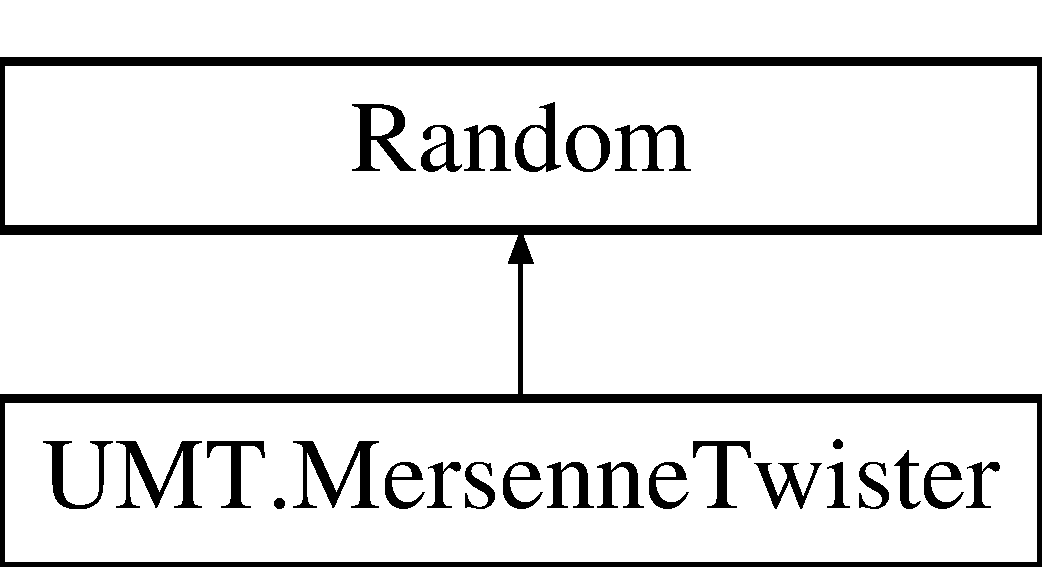
\includegraphics[height=2.000000cm]{class_u_m_t_1_1_mersenne_twister}
\end{center}
\end{figure}
\subsection*{Public Member Functions}
\begin{DoxyCompactItemize}
\item 
\hyperlink{class_u_m_t_1_1_mersenne_twister_a67f0b71e30df455fbcbba80c1d6acff9}{Mersenne\+Twister} (Int32 seed)
\begin{DoxyCompactList}\small\item\em Creates a new pseudo-\/random number generator with a given seed. \end{DoxyCompactList}\item 
\hyperlink{class_u_m_t_1_1_mersenne_twister_a9c574150f1f8df915497e4fce82de379}{Mersenne\+Twister} ()
\begin{DoxyCompactList}\small\item\em Creates a new pseudo-\/random number generator with a default seed. \end{DoxyCompactList}\item 
\hyperlink{class_u_m_t_1_1_mersenne_twister_ad23eef1dca9522daa6853e90a8b66ae0}{Mersenne\+Twister} (Int32\mbox{[}$\,$\mbox{]} init\+Key)
\begin{DoxyCompactList}\small\item\em Creates a pseudo-\/random number generator initialized with the given array. \end{DoxyCompactList}\item 
virtual U\+Int32 \hyperlink{class_u_m_t_1_1_mersenne_twister_a64e210aa86b47d3949e0e1f676b91565}{Next\+U\+Int32} ()
\begin{DoxyCompactList}\small\item\em Returns the next pseudo-\/random U\+Int32. \end{DoxyCompactList}\item 
virtual U\+Int32 \hyperlink{class_u_m_t_1_1_mersenne_twister_a9766d3a6c32e994ff8e698f7e500365a}{Next\+U\+Int32} (U\+Int32 max\+Value)
\begin{DoxyCompactList}\small\item\em Returns the next pseudo-\/random U\+Int32 up to {\itshape max\+Value} . \end{DoxyCompactList}\item 
virtual U\+Int32 \hyperlink{class_u_m_t_1_1_mersenne_twister_a965c38b14f0936c9b2af279a5f385108}{Next\+U\+Int32} (U\+Int32 min\+Value, U\+Int32 max\+Value)
\begin{DoxyCompactList}\small\item\em Returns the next pseudo-\/random U\+Int32 at least {\itshape min\+Value}  and up to {\itshape max\+Value} . \end{DoxyCompactList}\item 
override Int32 \hyperlink{class_u_m_t_1_1_mersenne_twister_af7c3a3d4b93537fbd72385518831000a}{Next} ()
\begin{DoxyCompactList}\small\item\em Returns the next pseudo-\/random Int32. \end{DoxyCompactList}\item 
override Int32 \hyperlink{class_u_m_t_1_1_mersenne_twister_a27a85323408740c511d5e71f887df796}{Next} (Int32 max\+Value)
\begin{DoxyCompactList}\small\item\em Returns the next pseudo-\/random Int32 up to {\itshape max\+Value} . \end{DoxyCompactList}\item 
override Int32 \hyperlink{class_u_m_t_1_1_mersenne_twister_a6e3aec9cc93283cfa10e896320f2d4c3}{Next} (Int32 min\+Value, Int32 max\+Value)
\begin{DoxyCompactList}\small\item\em Returns the next pseudo-\/random Int32 at least {\itshape min\+Value}  and up to {\itshape max\+Value} . \end{DoxyCompactList}\item 
override void \hyperlink{class_u_m_t_1_1_mersenne_twister_a33c4f7a3b84aecc1d7d3fb7ef198ac8b}{Next\+Bytes} (Byte\mbox{[}$\,$\mbox{]} buffer)
\begin{DoxyCompactList}\small\item\em Fills a buffer with pseudo-\/random bytes. \end{DoxyCompactList}\item 
override Double \hyperlink{class_u_m_t_1_1_mersenne_twister_a29216ecb75ec2fee71cb7542e1ffb5ab}{Next\+Double} ()
\begin{DoxyCompactList}\small\item\em Returns the next pseudo-\/random Double value. \end{DoxyCompactList}\item 
Double \hyperlink{class_u_m_t_1_1_mersenne_twister_a35074f09a2ce3c28af7683c360495de6}{Next\+Double} (Boolean include\+One)
\begin{DoxyCompactList}\small\item\em Returns a pseudo-\/random number greater than or equal to zero, and either strictly less than one, or less than or equal to one, depending on the value of the given parameter. \end{DoxyCompactList}\item 
Double \hyperlink{class_u_m_t_1_1_mersenne_twister_af663fc97c8f89da2c7484f2160bdd087}{Next\+Double\+Positive} ()
\begin{DoxyCompactList}\small\item\em Returns a pseudo-\/random number greater than 0.\+0 and less than 1.\+0. \end{DoxyCompactList}\item 
Single \hyperlink{class_u_m_t_1_1_mersenne_twister_abc37a49f3c72309e0ad61261f65cf6a2}{Next\+Single} ()
\begin{DoxyCompactList}\small\item\em Returns a pseudo-\/random number between 0.\+0 and 1.\+0. \end{DoxyCompactList}\item 
Single \hyperlink{class_u_m_t_1_1_mersenne_twister_aaba6c5b81f5697b14edc19f923576b1e}{Next\+Single} (Boolean include\+One)
\begin{DoxyCompactList}\small\item\em Returns a pseudo-\/random number greater than or equal to zero, and either strictly less than one, or less than or equal to one, depending on the value of the given boolean parameter. \end{DoxyCompactList}\item 
Single \hyperlink{class_u_m_t_1_1_mersenne_twister_a3770994cf65ccac5570ffa2291d15a16}{Next\+Single\+Positive} ()
\begin{DoxyCompactList}\small\item\em Returns a pseudo-\/random number greater than 0.\+0 and less than 1.\+0. \end{DoxyCompactList}\end{DoxyCompactItemize}
\subsection*{Protected Member Functions}
\begin{DoxyCompactItemize}
\item 
U\+Int32 \hyperlink{class_u_m_t_1_1_mersenne_twister_a6a5bd3b3327bce890c8a6456fe8d1207}{Generate\+U\+Int32} ()
\begin{DoxyCompactList}\small\item\em Generates a new pseudo-\/random U\+Int32. \end{DoxyCompactList}\end{DoxyCompactItemize}


\subsection{Detailed Description}
Generates pseudo-\/random numbers using the Mersenne Twister algorithm. 

See \href{http://www.math.sci.hiroshima-u.ac.jp/~m-mat/MT/emt.html}{\tt http\+://www.\+math.\+sci.\+hiroshima-\/u.\+ac.\+jp/$\sim$m-\/mat/\+M\+T/emt.\+html} for details on the algorithm. 

\subsection{Constructor \& Destructor Documentation}
\hypertarget{class_u_m_t_1_1_mersenne_twister_a67f0b71e30df455fbcbba80c1d6acff9}{\index{U\+M\+T\+::\+Mersenne\+Twister@{U\+M\+T\+::\+Mersenne\+Twister}!Mersenne\+Twister@{Mersenne\+Twister}}
\index{Mersenne\+Twister@{Mersenne\+Twister}!U\+M\+T\+::\+Mersenne\+Twister@{U\+M\+T\+::\+Mersenne\+Twister}}
\subsubsection[{Mersenne\+Twister}]{\setlength{\rightskip}{0pt plus 5cm}U\+M\+T.\+Mersenne\+Twister.\+Mersenne\+Twister (
\begin{DoxyParamCaption}
\item[{Int32}]{seed}
\end{DoxyParamCaption}
)\hspace{0.3cm}{\ttfamily [inline]}}}\label{class_u_m_t_1_1_mersenne_twister_a67f0b71e30df455fbcbba80c1d6acff9}


Creates a new pseudo-\/random number generator with a given seed. 


\begin{DoxyParams}{Parameters}
{\em seed} & A value to use as a seed.\\
\hline
\end{DoxyParams}
\hypertarget{class_u_m_t_1_1_mersenne_twister_a9c574150f1f8df915497e4fce82de379}{\index{U\+M\+T\+::\+Mersenne\+Twister@{U\+M\+T\+::\+Mersenne\+Twister}!Mersenne\+Twister@{Mersenne\+Twister}}
\index{Mersenne\+Twister@{Mersenne\+Twister}!U\+M\+T\+::\+Mersenne\+Twister@{U\+M\+T\+::\+Mersenne\+Twister}}
\subsubsection[{Mersenne\+Twister}]{\setlength{\rightskip}{0pt plus 5cm}U\+M\+T.\+Mersenne\+Twister.\+Mersenne\+Twister (
\begin{DoxyParamCaption}
{}
\end{DoxyParamCaption}
)\hspace{0.3cm}{\ttfamily [inline]}}}\label{class_u_m_t_1_1_mersenne_twister_a9c574150f1f8df915497e4fce82de379}


Creates a new pseudo-\/random number generator with a default seed. 

{\ttfamily new System.\+Random().Random.\+Next()} is used for the seed. \hypertarget{class_u_m_t_1_1_mersenne_twister_ad23eef1dca9522daa6853e90a8b66ae0}{\index{U\+M\+T\+::\+Mersenne\+Twister@{U\+M\+T\+::\+Mersenne\+Twister}!Mersenne\+Twister@{Mersenne\+Twister}}
\index{Mersenne\+Twister@{Mersenne\+Twister}!U\+M\+T\+::\+Mersenne\+Twister@{U\+M\+T\+::\+Mersenne\+Twister}}
\subsubsection[{Mersenne\+Twister}]{\setlength{\rightskip}{0pt plus 5cm}U\+M\+T.\+Mersenne\+Twister.\+Mersenne\+Twister (
\begin{DoxyParamCaption}
\item[{Int32\mbox{[}$\,$\mbox{]}}]{init\+Key}
\end{DoxyParamCaption}
)\hspace{0.3cm}{\ttfamily [inline]}}}\label{class_u_m_t_1_1_mersenne_twister_ad23eef1dca9522daa6853e90a8b66ae0}


Creates a pseudo-\/random number generator initialized with the given array. 


\begin{DoxyParams}{Parameters}
{\em init\+Key} & The array for initializing keys.\\
\hline
\end{DoxyParams}


\subsection{Member Function Documentation}
\hypertarget{class_u_m_t_1_1_mersenne_twister_a6a5bd3b3327bce890c8a6456fe8d1207}{\index{U\+M\+T\+::\+Mersenne\+Twister@{U\+M\+T\+::\+Mersenne\+Twister}!Generate\+U\+Int32@{Generate\+U\+Int32}}
\index{Generate\+U\+Int32@{Generate\+U\+Int32}!U\+M\+T\+::\+Mersenne\+Twister@{U\+M\+T\+::\+Mersenne\+Twister}}
\subsubsection[{Generate\+U\+Int32}]{\setlength{\rightskip}{0pt plus 5cm}U\+Int32 U\+M\+T.\+Mersenne\+Twister.\+Generate\+U\+Int32 (
\begin{DoxyParamCaption}
{}
\end{DoxyParamCaption}
)\hspace{0.3cm}{\ttfamily [inline]}, {\ttfamily [protected]}}}\label{class_u_m_t_1_1_mersenne_twister_a6a5bd3b3327bce890c8a6456fe8d1207}


Generates a new pseudo-\/random U\+Int32. 

\begin{DoxyReturn}{Returns}
A pseudo-\/random U\+Int32.
\end{DoxyReturn}
\hypertarget{class_u_m_t_1_1_mersenne_twister_af7c3a3d4b93537fbd72385518831000a}{\index{U\+M\+T\+::\+Mersenne\+Twister@{U\+M\+T\+::\+Mersenne\+Twister}!Next@{Next}}
\index{Next@{Next}!U\+M\+T\+::\+Mersenne\+Twister@{U\+M\+T\+::\+Mersenne\+Twister}}
\subsubsection[{Next}]{\setlength{\rightskip}{0pt plus 5cm}override Int32 U\+M\+T.\+Mersenne\+Twister.\+Next (
\begin{DoxyParamCaption}
{}
\end{DoxyParamCaption}
)\hspace{0.3cm}{\ttfamily [inline]}}}\label{class_u_m_t_1_1_mersenne_twister_af7c3a3d4b93537fbd72385518831000a}


Returns the next pseudo-\/random Int32. 

\begin{DoxyReturn}{Returns}
A pseudo-\/random Int32 value.
\end{DoxyReturn}
\hypertarget{class_u_m_t_1_1_mersenne_twister_a27a85323408740c511d5e71f887df796}{\index{U\+M\+T\+::\+Mersenne\+Twister@{U\+M\+T\+::\+Mersenne\+Twister}!Next@{Next}}
\index{Next@{Next}!U\+M\+T\+::\+Mersenne\+Twister@{U\+M\+T\+::\+Mersenne\+Twister}}
\subsubsection[{Next}]{\setlength{\rightskip}{0pt plus 5cm}override Int32 U\+M\+T.\+Mersenne\+Twister.\+Next (
\begin{DoxyParamCaption}
\item[{Int32}]{max\+Value}
\end{DoxyParamCaption}
)\hspace{0.3cm}{\ttfamily [inline]}}}\label{class_u_m_t_1_1_mersenne_twister_a27a85323408740c511d5e71f887df796}


Returns the next pseudo-\/random Int32 up to {\itshape max\+Value} . 


\begin{DoxyParams}{Parameters}
{\em max\+Value} & The maximum value of the pseudo-\/random number to create.\\
\hline
\end{DoxyParams}
\begin{DoxyReturn}{Returns}
A pseudo-\/random Int32 value which is at most {\itshape max\+Value} . 
\end{DoxyReturn}

\begin{DoxyExceptions}{Exceptions}
{\em Argument\+Out\+Of\+Range\+Exception} & When {\itshape max\+Value}  $<$ 0. \\
\hline
\end{DoxyExceptions}
\hypertarget{class_u_m_t_1_1_mersenne_twister_a6e3aec9cc93283cfa10e896320f2d4c3}{\index{U\+M\+T\+::\+Mersenne\+Twister@{U\+M\+T\+::\+Mersenne\+Twister}!Next@{Next}}
\index{Next@{Next}!U\+M\+T\+::\+Mersenne\+Twister@{U\+M\+T\+::\+Mersenne\+Twister}}
\subsubsection[{Next}]{\setlength{\rightskip}{0pt plus 5cm}override Int32 U\+M\+T.\+Mersenne\+Twister.\+Next (
\begin{DoxyParamCaption}
\item[{Int32}]{min\+Value, }
\item[{Int32}]{max\+Value}
\end{DoxyParamCaption}
)\hspace{0.3cm}{\ttfamily [inline]}}}\label{class_u_m_t_1_1_mersenne_twister_a6e3aec9cc93283cfa10e896320f2d4c3}


Returns the next pseudo-\/random Int32 at least {\itshape min\+Value}  and up to {\itshape max\+Value} . 


\begin{DoxyParams}{Parameters}
{\em min\+Value} & The minimum value of the pseudo-\/random number to create.\\
\hline
{\em max\+Value} & The maximum value of the pseudo-\/random number to create.\\
\hline
\end{DoxyParams}
\begin{DoxyReturn}{Returns}
A pseudo-\/random Int32 value which is at least {\itshape min\+Value}  and at most {\itshape max\+Value} .
\end{DoxyReturn}

\begin{DoxyExceptions}{Exceptions}
{\em Argument\+Out\+Of\+Range\+Exception} & If {\ttfamily {\itshape min\+Value}  $>$= {\itshape max\+Value} }. \\
\hline
\end{DoxyExceptions}
\hypertarget{class_u_m_t_1_1_mersenne_twister_a33c4f7a3b84aecc1d7d3fb7ef198ac8b}{\index{U\+M\+T\+::\+Mersenne\+Twister@{U\+M\+T\+::\+Mersenne\+Twister}!Next\+Bytes@{Next\+Bytes}}
\index{Next\+Bytes@{Next\+Bytes}!U\+M\+T\+::\+Mersenne\+Twister@{U\+M\+T\+::\+Mersenne\+Twister}}
\subsubsection[{Next\+Bytes}]{\setlength{\rightskip}{0pt plus 5cm}override void U\+M\+T.\+Mersenne\+Twister.\+Next\+Bytes (
\begin{DoxyParamCaption}
\item[{Byte\mbox{[}$\,$\mbox{]}}]{buffer}
\end{DoxyParamCaption}
)\hspace{0.3cm}{\ttfamily [inline]}}}\label{class_u_m_t_1_1_mersenne_twister_a33c4f7a3b84aecc1d7d3fb7ef198ac8b}


Fills a buffer with pseudo-\/random bytes. 


\begin{DoxyParams}{Parameters}
{\em buffer} & The buffer to fill.\\
\hline
\end{DoxyParams}

\begin{DoxyExceptions}{Exceptions}
{\em Argument\+Null\+Exception} & If {\ttfamily {\itshape buffer}  == }. \\
\hline
\end{DoxyExceptions}
\hypertarget{class_u_m_t_1_1_mersenne_twister_a29216ecb75ec2fee71cb7542e1ffb5ab}{\index{U\+M\+T\+::\+Mersenne\+Twister@{U\+M\+T\+::\+Mersenne\+Twister}!Next\+Double@{Next\+Double}}
\index{Next\+Double@{Next\+Double}!U\+M\+T\+::\+Mersenne\+Twister@{U\+M\+T\+::\+Mersenne\+Twister}}
\subsubsection[{Next\+Double}]{\setlength{\rightskip}{0pt plus 5cm}override Double U\+M\+T.\+Mersenne\+Twister.\+Next\+Double (
\begin{DoxyParamCaption}
{}
\end{DoxyParamCaption}
)\hspace{0.3cm}{\ttfamily [inline]}}}\label{class_u_m_t_1_1_mersenne_twister_a29216ecb75ec2fee71cb7542e1ffb5ab}


Returns the next pseudo-\/random Double value. 

\begin{DoxyReturn}{Returns}
A pseudo-\/random double floating point value.
\end{DoxyReturn}


There are two common ways to create a double floating point using M\+T19937\+: using \hyperlink{class_u_m_t_1_1_mersenne_twister_a6a5bd3b3327bce890c8a6456fe8d1207}{Generate\+U\+Int32} and dividing by 0x\+F\+F\+F\+F\+F\+F\+F\+F + 1, or else generating two double words and shifting the first by 26 bits and adding the second. 

In a newer measurement of the randomness of M\+T19937 published in the journal \char`\"{}\+Monte Carlo Methods and Applications, Vol. 12, No. 5-\/6, pp. 385 � 393 (2006)\char`\"{} entitled \char`\"{}\+A Repetition Test for Pseudo-\/\+Random Number Generators\char`\"{}, it was found that the 32-\/bit version of generating a double fails at the 95\% confidence level when measuring for expected repetitions of a particular number in a sequence of numbers generated by the algorithm. 

Due to this, the 53-\/bit method is implemented here and the 32-\/bit method of generating a double is not. If, for some reason, the 32-\/bit method is needed, it can be generated by the following\+: 
\begin{DoxyCode}
(Double)\hyperlink{class_u_m_t_1_1_mersenne_twister_a64e210aa86b47d3949e0e1f676b91565}{NextUInt32}() / ((UInt64)UInt32.MaxValue + 1);
\end{DoxyCode}
 \hypertarget{class_u_m_t_1_1_mersenne_twister_a35074f09a2ce3c28af7683c360495de6}{\index{U\+M\+T\+::\+Mersenne\+Twister@{U\+M\+T\+::\+Mersenne\+Twister}!Next\+Double@{Next\+Double}}
\index{Next\+Double@{Next\+Double}!U\+M\+T\+::\+Mersenne\+Twister@{U\+M\+T\+::\+Mersenne\+Twister}}
\subsubsection[{Next\+Double}]{\setlength{\rightskip}{0pt plus 5cm}Double U\+M\+T.\+Mersenne\+Twister.\+Next\+Double (
\begin{DoxyParamCaption}
\item[{Boolean}]{include\+One}
\end{DoxyParamCaption}
)\hspace{0.3cm}{\ttfamily [inline]}}}\label{class_u_m_t_1_1_mersenne_twister_a35074f09a2ce3c28af7683c360495de6}


Returns a pseudo-\/random number greater than or equal to zero, and either strictly less than one, or less than or equal to one, depending on the value of the given parameter. 


\begin{DoxyParams}{Parameters}
{\em include\+One} & If , the pseudo-\/random number returned will be less than or equal to one; otherwise, the pseudo-\/random number returned will be strictly less than one. \\
\hline
\end{DoxyParams}
\begin{DoxyReturn}{Returns}
If {\itshape include\+One}  is , this method returns a double-\/precision pseudo-\/random number greater than or equal to zero, and less than or equal to one. If {\itshape include\+One}  is , this method returns a double-\/precision pseudo-\/random number greater than or equal to zero and strictly less than one. 
\end{DoxyReturn}
\hypertarget{class_u_m_t_1_1_mersenne_twister_af663fc97c8f89da2c7484f2160bdd087}{\index{U\+M\+T\+::\+Mersenne\+Twister@{U\+M\+T\+::\+Mersenne\+Twister}!Next\+Double\+Positive@{Next\+Double\+Positive}}
\index{Next\+Double\+Positive@{Next\+Double\+Positive}!U\+M\+T\+::\+Mersenne\+Twister@{U\+M\+T\+::\+Mersenne\+Twister}}
\subsubsection[{Next\+Double\+Positive}]{\setlength{\rightskip}{0pt plus 5cm}Double U\+M\+T.\+Mersenne\+Twister.\+Next\+Double\+Positive (
\begin{DoxyParamCaption}
{}
\end{DoxyParamCaption}
)\hspace{0.3cm}{\ttfamily [inline]}}}\label{class_u_m_t_1_1_mersenne_twister_af663fc97c8f89da2c7484f2160bdd087}


Returns a pseudo-\/random number greater than 0.\+0 and less than 1.\+0. 

\begin{DoxyReturn}{Returns}
A pseudo-\/random number greater than 0.\+0 and less than 1.\+0.
\end{DoxyReturn}
\hypertarget{class_u_m_t_1_1_mersenne_twister_abc37a49f3c72309e0ad61261f65cf6a2}{\index{U\+M\+T\+::\+Mersenne\+Twister@{U\+M\+T\+::\+Mersenne\+Twister}!Next\+Single@{Next\+Single}}
\index{Next\+Single@{Next\+Single}!U\+M\+T\+::\+Mersenne\+Twister@{U\+M\+T\+::\+Mersenne\+Twister}}
\subsubsection[{Next\+Single}]{\setlength{\rightskip}{0pt plus 5cm}Single U\+M\+T.\+Mersenne\+Twister.\+Next\+Single (
\begin{DoxyParamCaption}
{}
\end{DoxyParamCaption}
)\hspace{0.3cm}{\ttfamily [inline]}}}\label{class_u_m_t_1_1_mersenne_twister_abc37a49f3c72309e0ad61261f65cf6a2}


Returns a pseudo-\/random number between 0.\+0 and 1.\+0. 

\begin{DoxyReturn}{Returns}
A single-\/precision floating point number greater than or equal to 0.\+0, and less than 1.\+0. 
\end{DoxyReturn}
\hypertarget{class_u_m_t_1_1_mersenne_twister_aaba6c5b81f5697b14edc19f923576b1e}{\index{U\+M\+T\+::\+Mersenne\+Twister@{U\+M\+T\+::\+Mersenne\+Twister}!Next\+Single@{Next\+Single}}
\index{Next\+Single@{Next\+Single}!U\+M\+T\+::\+Mersenne\+Twister@{U\+M\+T\+::\+Mersenne\+Twister}}
\subsubsection[{Next\+Single}]{\setlength{\rightskip}{0pt plus 5cm}Single U\+M\+T.\+Mersenne\+Twister.\+Next\+Single (
\begin{DoxyParamCaption}
\item[{Boolean}]{include\+One}
\end{DoxyParamCaption}
)\hspace{0.3cm}{\ttfamily [inline]}}}\label{class_u_m_t_1_1_mersenne_twister_aaba6c5b81f5697b14edc19f923576b1e}


Returns a pseudo-\/random number greater than or equal to zero, and either strictly less than one, or less than or equal to one, depending on the value of the given boolean parameter. 


\begin{DoxyParams}{Parameters}
{\em include\+One} & If , the pseudo-\/random number returned will be less than or equal to one; otherwise, the pseudo-\/random number returned will be strictly less than one. \\
\hline
\end{DoxyParams}
\begin{DoxyReturn}{Returns}
If {\itshape include\+One}  is , this method returns a single-\/precision pseudo-\/random number greater than or equal to zero, and less than or equal to one. If {\itshape include\+One}  is , this method returns a single-\/precision pseudo-\/random number greater than or equal to zero and strictly less than one. 
\end{DoxyReturn}
\hypertarget{class_u_m_t_1_1_mersenne_twister_a3770994cf65ccac5570ffa2291d15a16}{\index{U\+M\+T\+::\+Mersenne\+Twister@{U\+M\+T\+::\+Mersenne\+Twister}!Next\+Single\+Positive@{Next\+Single\+Positive}}
\index{Next\+Single\+Positive@{Next\+Single\+Positive}!U\+M\+T\+::\+Mersenne\+Twister@{U\+M\+T\+::\+Mersenne\+Twister}}
\subsubsection[{Next\+Single\+Positive}]{\setlength{\rightskip}{0pt plus 5cm}Single U\+M\+T.\+Mersenne\+Twister.\+Next\+Single\+Positive (
\begin{DoxyParamCaption}
{}
\end{DoxyParamCaption}
)\hspace{0.3cm}{\ttfamily [inline]}}}\label{class_u_m_t_1_1_mersenne_twister_a3770994cf65ccac5570ffa2291d15a16}


Returns a pseudo-\/random number greater than 0.\+0 and less than 1.\+0. 

\begin{DoxyReturn}{Returns}
A pseudo-\/random number greater than 0.\+0 and less than 1.\+0.
\end{DoxyReturn}
\hypertarget{class_u_m_t_1_1_mersenne_twister_a64e210aa86b47d3949e0e1f676b91565}{\index{U\+M\+T\+::\+Mersenne\+Twister@{U\+M\+T\+::\+Mersenne\+Twister}!Next\+U\+Int32@{Next\+U\+Int32}}
\index{Next\+U\+Int32@{Next\+U\+Int32}!U\+M\+T\+::\+Mersenne\+Twister@{U\+M\+T\+::\+Mersenne\+Twister}}
\subsubsection[{Next\+U\+Int32}]{\setlength{\rightskip}{0pt plus 5cm}virtual U\+Int32 U\+M\+T.\+Mersenne\+Twister.\+Next\+U\+Int32 (
\begin{DoxyParamCaption}
{}
\end{DoxyParamCaption}
)\hspace{0.3cm}{\ttfamily [inline]}, {\ttfamily [virtual]}}}\label{class_u_m_t_1_1_mersenne_twister_a64e210aa86b47d3949e0e1f676b91565}


Returns the next pseudo-\/random U\+Int32. 

\begin{DoxyReturn}{Returns}
A pseudo-\/random U\+Int32 value.
\end{DoxyReturn}
\hypertarget{class_u_m_t_1_1_mersenne_twister_a9766d3a6c32e994ff8e698f7e500365a}{\index{U\+M\+T\+::\+Mersenne\+Twister@{U\+M\+T\+::\+Mersenne\+Twister}!Next\+U\+Int32@{Next\+U\+Int32}}
\index{Next\+U\+Int32@{Next\+U\+Int32}!U\+M\+T\+::\+Mersenne\+Twister@{U\+M\+T\+::\+Mersenne\+Twister}}
\subsubsection[{Next\+U\+Int32}]{\setlength{\rightskip}{0pt plus 5cm}virtual U\+Int32 U\+M\+T.\+Mersenne\+Twister.\+Next\+U\+Int32 (
\begin{DoxyParamCaption}
\item[{U\+Int32}]{max\+Value}
\end{DoxyParamCaption}
)\hspace{0.3cm}{\ttfamily [inline]}, {\ttfamily [virtual]}}}\label{class_u_m_t_1_1_mersenne_twister_a9766d3a6c32e994ff8e698f7e500365a}


Returns the next pseudo-\/random U\+Int32 up to {\itshape max\+Value} . 


\begin{DoxyParams}{Parameters}
{\em max\+Value} & The maximum value of the pseudo-\/random number to create. \\
\hline
\end{DoxyParams}
\begin{DoxyReturn}{Returns}
A pseudo-\/random U\+Int32 value which is at most {\itshape max\+Value} . 
\end{DoxyReturn}
\hypertarget{class_u_m_t_1_1_mersenne_twister_a965c38b14f0936c9b2af279a5f385108}{\index{U\+M\+T\+::\+Mersenne\+Twister@{U\+M\+T\+::\+Mersenne\+Twister}!Next\+U\+Int32@{Next\+U\+Int32}}
\index{Next\+U\+Int32@{Next\+U\+Int32}!U\+M\+T\+::\+Mersenne\+Twister@{U\+M\+T\+::\+Mersenne\+Twister}}
\subsubsection[{Next\+U\+Int32}]{\setlength{\rightskip}{0pt plus 5cm}virtual U\+Int32 U\+M\+T.\+Mersenne\+Twister.\+Next\+U\+Int32 (
\begin{DoxyParamCaption}
\item[{U\+Int32}]{min\+Value, }
\item[{U\+Int32}]{max\+Value}
\end{DoxyParamCaption}
)\hspace{0.3cm}{\ttfamily [inline]}, {\ttfamily [virtual]}}}\label{class_u_m_t_1_1_mersenne_twister_a965c38b14f0936c9b2af279a5f385108}


Returns the next pseudo-\/random U\+Int32 at least {\itshape min\+Value}  and up to {\itshape max\+Value} . 


\begin{DoxyParams}{Parameters}
{\em min\+Value} & The minimum value of the pseudo-\/random number to create.\\
\hline
{\em max\+Value} & The maximum value of the pseudo-\/random number to create.\\
\hline
\end{DoxyParams}
\begin{DoxyReturn}{Returns}
A pseudo-\/random U\+Int32 value which is at least {\itshape min\+Value}  and at most {\itshape max\+Value} . 
\end{DoxyReturn}

\begin{DoxyExceptions}{Exceptions}
{\em Argument\+Out\+Of\+Range\+Exception} & If {\ttfamily {\itshape min\+Value}  $>$= {\itshape max\+Value} }. \\
\hline
\end{DoxyExceptions}


The documentation for this class was generated from the following file\+:\begin{DoxyCompactItemize}
\item 
/\+Users/tucano/\+Documents/\+Devel/\+Unity/\+Unity\+Projects/\+M\+T\+Random/\+Assets/\+M\+T\+Random/\+Scripts/lib/Mersenne\+Twister.\+cs\end{DoxyCompactItemize}

\hypertarget{class_m_t_random}{\section{M\+T\+Random Class Reference}
\label{class_m_t_random}\index{M\+T\+Random@{M\+T\+Random}}
}


M\+T random interface.  


\subsection*{Public Types}
\begin{DoxyCompactItemize}
\item 
\hypertarget{class_m_t_random_a0d2e3a1fc694095ed0cdb5fdd0cf1fb9}{enum {\bfseries Normalization} \{ {\bfseries S\+T\+D\+N\+O\+R\+M\+A\+L} = 0, 
{\bfseries P\+O\+W\+E\+R\+L\+A\+W} = 1
 \}}\label{class_m_t_random_a0d2e3a1fc694095ed0cdb5fdd0cf1fb9}

\end{DoxyCompactItemize}
\subsection*{Public Member Functions}
\begin{DoxyCompactItemize}
\item 
\hyperlink{class_m_t_random_af0a395715fa76193de56b49a98bef41d}{M\+T\+Random} ()
\begin{DoxyCompactList}\small\item\em Initializes a new instance of the \hyperlink{class_m_t_random}{M\+T\+Random} class. \end{DoxyCompactList}\item 
\hyperlink{class_m_t_random_a6c49868b07fd6300f99877fdd7115997}{M\+T\+Random} (int seed)
\begin{DoxyCompactList}\small\item\em Initializes a new instance of the \hyperlink{class_m_t_random}{M\+T\+Random} class. \end{DoxyCompactList}\item 
\hyperlink{class_m_t_random_a2ca2ad75c477b008d70380f9fd03c9a6}{M\+T\+Random} (string phrase)
\begin{DoxyCompactList}\small\item\em Initializes a new instance of the \hyperlink{class_m_t_random}{M\+T\+Random} class. \end{DoxyCompactList}\item 
float \hyperlink{class_m_t_random_ad0cc614bc3b023f2036e6a0bc5532763}{value} ()
\begin{DoxyCompactList}\small\item\em Returns a pseudo-\/random number between 0.\+0 \mbox{[}inclusive\mbox{]} and 1.\+0 \mbox{[}inclusive\mbox{]} (Read Only). \end{DoxyCompactList}\item 
float \hyperlink{class_m_t_random_a6406f326587e9cb869277f97ffa56f83}{value} (bool include\+One)
\begin{DoxyCompactList}\small\item\em Returns a pseudo-\/random number greater than or equal to zero, and either strictly less than one, or less than or equal to one, depending on the value of the given boolean parameter. \end{DoxyCompactList}\item 
float \hyperlink{class_m_t_random_a56cf43aef8ed6504c5c4d8fd379704df}{value\+Norm} (float temperature)
\begin{DoxyCompactList}\small\item\em Returns a pseudo-\/random number between 0.\+0 \mbox{[}inclusive\mbox{]} and 1.\+0 \mbox{[}inclusive\mbox{]} (Read Only). Normalized around 0.\+5 with {\itshape temperature} . \end{DoxyCompactList}\item 
float \hyperlink{class_m_t_random_aef2e82a3345b85fdc075476b2c1f81de}{value\+Power} (float temperature)
\begin{DoxyCompactList}\small\item\em Returns a pseudo-\/random number in Power Law distribution between 0.\+0 \mbox{[}inclusive\mbox{]} and 1.\+0 \mbox{[}inclusive\mbox{]} (Read Only). \end{DoxyCompactList}\item 
float \hyperlink{class_m_t_random_a5bfa094b57244746389d4ab89284c8a7}{value\+Poisson} (float lambda)
\begin{DoxyCompactList}\small\item\em Returns a pseudo-\/random number in Poisson distribution between 0.\+0 \mbox{[}inclusive\mbox{]} and 1.\+0 \mbox{[}inclusive\mbox{]} (Read Only). \end{DoxyCompactList}\item 
float \hyperlink{class_m_t_random_a0f9deae2e629a2e8a9164d7f53e35537}{value\+Exponential} (float lambda)
\begin{DoxyCompactList}\small\item\em Returns a pseudo-\/random number in Exponential distribution between 0.\+0 \mbox{[}inclusive\mbox{]} and 1.\+0 \mbox{[}inclusive\mbox{]} (Read Only). \end{DoxyCompactList}\item 
float \hyperlink{class_m_t_random_abbd3cdd52723d6540e1ec30ab105e31e}{value\+Gamma} (int order)
\begin{DoxyCompactList}\small\item\em Returns a pseudo-\/random number the gamma distribution. \end{DoxyCompactList}\item 
int \hyperlink{class_m_t_random_ab1d2aae9abe7a2d01a8a93ecb697248c}{Range} (int min, int max)
\begin{DoxyCompactList}\small\item\em Returns the next pseudo-\/random number integer between {\itshape min}  \mbox{[}inclusive\mbox{]} and {\itshape max}  \mbox{[}inclusive\mbox{]}. \end{DoxyCompactList}\item 
float \hyperlink{class_m_t_random_a3ffd8b27980f7f416d33c3823b0c2611}{Range} (float min, float max)
\begin{DoxyCompactList}\small\item\em Returns the next pseudo-\/random number integer between {\itshape min}  \mbox{[}inclusive\mbox{]} and {\itshape max}  \mbox{[}inclusive\mbox{]}. \end{DoxyCompactList}\item 
float \hyperlink{class_m_t_random_a67f0856b5501a37b3ec078fbf0096754}{Range\+Norm} (float min, float max, float temperature)
\begin{DoxyCompactList}\small\item\em Returns the next pseudo-\/random number integer between {\itshape min}  \mbox{[}inclusive\mbox{]} and {\itshape max}  \mbox{[}inclusive\mbox{]}. \end{DoxyCompactList}\item 
float \hyperlink{class_m_t_random_aa7ab0237fc962a1f63e0a90c24db2ed2}{Range\+Power} (float min, float max, float temperature)
\begin{DoxyCompactList}\small\item\em Returns the next pseudo-\/random number integer between {\itshape min}  \mbox{[}inclusive\mbox{]} and {\itshape max}  \mbox{[}inclusive\mbox{]}. in Power Law distribution \end{DoxyCompactList}\item 
Color \hyperlink{class_m_t_random_adf641ad01fbd3c27a38f3047e59eb45d}{color} ()
\begin{DoxyCompactList}\small\item\em Return the next pseudo-\/random number as a Color \end{DoxyCompactList}\item 
Color \hyperlink{class_m_t_random_ae3f6b4f17b19399861d75f877e24d4f7}{color} (float min, float max)
\begin{DoxyCompactList}\small\item\em Return the next pseudo-\/random number as a Color with a linear scale \mbox{[}0.\+0-\/1.\+0\mbox{]}. Use a range between {\itshape min}  \mbox{[}inclusive\mbox{]} and {\itshape max}  \mbox{[}inclusive\mbox{]} to reduce the color range. \end{DoxyCompactList}\item 
\hypertarget{class_m_t_random_a28394b9419cee95f3b7cef5b269ef6df}{Vector2 {\bfseries Point\+In\+A\+Square} ()}\label{class_m_t_random_a28394b9419cee95f3b7cef5b269ef6df}

\item 
\hypertarget{class_m_t_random_a7ce51ff0fde5d9f0a508bdaa528a830c}{Vector2 {\bfseries Point\+In\+A\+Square} (Normalization n, float t)}\label{class_m_t_random_a7ce51ff0fde5d9f0a508bdaa528a830c}

\item 
\hypertarget{class_m_t_random_ad91aa159280b36e6eafb6eb9638b1cc1}{Vector2 {\bfseries Point\+In\+A\+Circle} ()}\label{class_m_t_random_ad91aa159280b36e6eafb6eb9638b1cc1}

\item 
\hypertarget{class_m_t_random_a553c19d7dc936ccabc411b46dca83be3}{Vector2 {\bfseries Point\+In\+A\+Circle} (Normalization n, float t)}\label{class_m_t_random_a553c19d7dc936ccabc411b46dca83be3}

\item 
\hypertarget{class_m_t_random_a4ef4c9e90cbd576168827b38a92c12bd}{Vector2 {\bfseries Point\+In\+A\+Disk} ()}\label{class_m_t_random_a4ef4c9e90cbd576168827b38a92c12bd}

\item 
\hypertarget{class_m_t_random_a80193b6a2351fe862097479aad6eba24}{Vector2 {\bfseries Point\+In\+A\+Disk} (Normalization n, float t)}\label{class_m_t_random_a80193b6a2351fe862097479aad6eba24}

\item 
\hypertarget{class_m_t_random_a37ad054ace9ab2d9853e633618a0f841}{Vector3 {\bfseries Point\+In\+A\+Cube} ()}\label{class_m_t_random_a37ad054ace9ab2d9853e633618a0f841}

\item 
\hypertarget{class_m_t_random_ace356958f5a49e7fd57dfac834df576c}{Vector3 {\bfseries Point\+In\+A\+Cube} (Normalization n, float t)}\label{class_m_t_random_ace356958f5a49e7fd57dfac834df576c}

\item 
\hypertarget{class_m_t_random_a181c5763ec6fc54ce32b03e5e8b70999}{Vector3 {\bfseries Point\+On\+A\+Cube} ()}\label{class_m_t_random_a181c5763ec6fc54ce32b03e5e8b70999}

\item 
\hypertarget{class_m_t_random_a35b79e5690fc372501c9116db5d4edbf}{Vector3 {\bfseries Point\+On\+A\+Cube} (Normalization n, float t)}\label{class_m_t_random_a35b79e5690fc372501c9116db5d4edbf}

\item 
\hypertarget{class_m_t_random_a6af47a9f988ce9b163455b1abfb4e12d}{Vector3 {\bfseries Point\+On\+A\+Sphere} ()}\label{class_m_t_random_a6af47a9f988ce9b163455b1abfb4e12d}

\item 
\hypertarget{class_m_t_random_a8a4ffd8278d115d6b840b872a92cf6b4}{Vector3 {\bfseries Point\+In\+A\+Sphere} ()}\label{class_m_t_random_a8a4ffd8278d115d6b840b872a92cf6b4}

\item 
\hypertarget{class_m_t_random_ab3d4e8b9af933503afbd3640da7ae2ec}{Vector3 {\bfseries Point\+On\+Cap} (float spot\+Angle)}\label{class_m_t_random_ab3d4e8b9af933503afbd3640da7ae2ec}

\item 
\hypertarget{class_m_t_random_ad33764572f7d2aee6aa83e5b2539cc73}{Vector3 {\bfseries Point\+On\+Ring} (float inner\+Angle, float outer\+Angle)}\label{class_m_t_random_ad33764572f7d2aee6aa83e5b2539cc73}

\end{DoxyCompactItemize}
\subsection*{Static Public Member Functions}
\begin{DoxyCompactItemize}
\item 
static float \hyperlink{class_m_t_random_a2f08d7209bdcd77ed9598820497c6255}{Scale\+Float\+To\+Range} (float x, float new\+Min, float new\+Max, float old\+Min, float old\+Max)
\begin{DoxyCompactList}\small\item\em Scales the float to any range. \end{DoxyCompactList}\end{DoxyCompactItemize}


\subsection{Detailed Description}
M\+T random interface. 



\subsection{Constructor \& Destructor Documentation}
\hypertarget{class_m_t_random_af0a395715fa76193de56b49a98bef41d}{\index{M\+T\+Random@{M\+T\+Random}!M\+T\+Random@{M\+T\+Random}}
\index{M\+T\+Random@{M\+T\+Random}!M\+T\+Random@{M\+T\+Random}}
\subsubsection[{M\+T\+Random}]{\setlength{\rightskip}{0pt plus 5cm}M\+T\+Random.\+M\+T\+Random (
\begin{DoxyParamCaption}
{}
\end{DoxyParamCaption}
)\hspace{0.3cm}{\ttfamily [inline]}}}\label{class_m_t_random_af0a395715fa76193de56b49a98bef41d}


Initializes a new instance of the \hyperlink{class_m_t_random}{M\+T\+Random} class. 

\hypertarget{class_m_t_random_a6c49868b07fd6300f99877fdd7115997}{\index{M\+T\+Random@{M\+T\+Random}!M\+T\+Random@{M\+T\+Random}}
\index{M\+T\+Random@{M\+T\+Random}!M\+T\+Random@{M\+T\+Random}}
\subsubsection[{M\+T\+Random}]{\setlength{\rightskip}{0pt plus 5cm}M\+T\+Random.\+M\+T\+Random (
\begin{DoxyParamCaption}
\item[{int}]{seed}
\end{DoxyParamCaption}
)\hspace{0.3cm}{\ttfamily [inline]}}}\label{class_m_t_random_a6c49868b07fd6300f99877fdd7115997}


Initializes a new instance of the \hyperlink{class_m_t_random}{M\+T\+Random} class. 


\begin{DoxyParams}{Parameters}
{\em seed} & Seed.\\
\hline
\end{DoxyParams}
\hypertarget{class_m_t_random_a2ca2ad75c477b008d70380f9fd03c9a6}{\index{M\+T\+Random@{M\+T\+Random}!M\+T\+Random@{M\+T\+Random}}
\index{M\+T\+Random@{M\+T\+Random}!M\+T\+Random@{M\+T\+Random}}
\subsubsection[{M\+T\+Random}]{\setlength{\rightskip}{0pt plus 5cm}M\+T\+Random.\+M\+T\+Random (
\begin{DoxyParamCaption}
\item[{string}]{phrase}
\end{DoxyParamCaption}
)\hspace{0.3cm}{\ttfamily [inline]}}}\label{class_m_t_random_a2ca2ad75c477b008d70380f9fd03c9a6}


Initializes a new instance of the \hyperlink{class_m_t_random}{M\+T\+Random} class. 


\begin{DoxyParams}{Parameters}
{\em phrase} & Phrase.\\
\hline
\end{DoxyParams}


\subsection{Member Function Documentation}
\hypertarget{class_m_t_random_adf641ad01fbd3c27a38f3047e59eb45d}{\index{M\+T\+Random@{M\+T\+Random}!color@{color}}
\index{color@{color}!M\+T\+Random@{M\+T\+Random}}
\subsubsection[{color}]{\setlength{\rightskip}{0pt plus 5cm}Color M\+T\+Random.\+color (
\begin{DoxyParamCaption}
{}
\end{DoxyParamCaption}
)\hspace{0.3cm}{\ttfamily [inline]}}}\label{class_m_t_random_adf641ad01fbd3c27a38f3047e59eb45d}


Return the next pseudo-\/random number as a Color 

\hypertarget{class_m_t_random_ae3f6b4f17b19399861d75f877e24d4f7}{\index{M\+T\+Random@{M\+T\+Random}!color@{color}}
\index{color@{color}!M\+T\+Random@{M\+T\+Random}}
\subsubsection[{color}]{\setlength{\rightskip}{0pt plus 5cm}Color M\+T\+Random.\+color (
\begin{DoxyParamCaption}
\item[{float}]{min, }
\item[{float}]{max}
\end{DoxyParamCaption}
)\hspace{0.3cm}{\ttfamily [inline]}}}\label{class_m_t_random_ae3f6b4f17b19399861d75f877e24d4f7}


Return the next pseudo-\/random number as a Color with a linear scale \mbox{[}0.\+0-\/1.\+0\mbox{]}. Use a range between {\itshape min}  \mbox{[}inclusive\mbox{]} and {\itshape max}  \mbox{[}inclusive\mbox{]} to reduce the color range. 


\begin{DoxyParams}{Parameters}
{\em min} & Minimum.\\
\hline
{\em max} & Max.\\
\hline
\end{DoxyParams}
\hypertarget{class_m_t_random_ab1d2aae9abe7a2d01a8a93ecb697248c}{\index{M\+T\+Random@{M\+T\+Random}!Range@{Range}}
\index{Range@{Range}!M\+T\+Random@{M\+T\+Random}}
\subsubsection[{Range}]{\setlength{\rightskip}{0pt plus 5cm}int M\+T\+Random.\+Range (
\begin{DoxyParamCaption}
\item[{int}]{min, }
\item[{int}]{max}
\end{DoxyParamCaption}
)\hspace{0.3cm}{\ttfamily [inline]}}}\label{class_m_t_random_ab1d2aae9abe7a2d01a8a93ecb697248c}


Returns the next pseudo-\/random number integer between {\itshape min}  \mbox{[}inclusive\mbox{]} and {\itshape max}  \mbox{[}inclusive\mbox{]}. 


\begin{DoxyParams}{Parameters}
{\em min} & Minimum.\\
\hline
{\em max} & Maximum.\\
\hline
\end{DoxyParams}
\hypertarget{class_m_t_random_a3ffd8b27980f7f416d33c3823b0c2611}{\index{M\+T\+Random@{M\+T\+Random}!Range@{Range}}
\index{Range@{Range}!M\+T\+Random@{M\+T\+Random}}
\subsubsection[{Range}]{\setlength{\rightskip}{0pt plus 5cm}float M\+T\+Random.\+Range (
\begin{DoxyParamCaption}
\item[{float}]{min, }
\item[{float}]{max}
\end{DoxyParamCaption}
)\hspace{0.3cm}{\ttfamily [inline]}}}\label{class_m_t_random_a3ffd8b27980f7f416d33c3823b0c2611}


Returns the next pseudo-\/random number integer between {\itshape min}  \mbox{[}inclusive\mbox{]} and {\itshape max}  \mbox{[}inclusive\mbox{]}. 


\begin{DoxyParams}{Parameters}
{\em min} & Minimum.\\
\hline
{\em max} & Maximum.\\
\hline
\end{DoxyParams}
\hypertarget{class_m_t_random_a67f0856b5501a37b3ec078fbf0096754}{\index{M\+T\+Random@{M\+T\+Random}!Range\+Norm@{Range\+Norm}}
\index{Range\+Norm@{Range\+Norm}!M\+T\+Random@{M\+T\+Random}}
\subsubsection[{Range\+Norm}]{\setlength{\rightskip}{0pt plus 5cm}float M\+T\+Random.\+Range\+Norm (
\begin{DoxyParamCaption}
\item[{float}]{min, }
\item[{float}]{max, }
\item[{float}]{temperature}
\end{DoxyParamCaption}
)\hspace{0.3cm}{\ttfamily [inline]}}}\label{class_m_t_random_a67f0856b5501a37b3ec078fbf0096754}


Returns the next pseudo-\/random number integer between {\itshape min}  \mbox{[}inclusive\mbox{]} and {\itshape max}  \mbox{[}inclusive\mbox{]}. 


\begin{DoxyParams}{Parameters}
{\em min} & Minimum.\\
\hline
{\em max} & Maximum.\\
\hline
{\em temperature} & Temperature.\\
\hline
\end{DoxyParams}
\hypertarget{class_m_t_random_aa7ab0237fc962a1f63e0a90c24db2ed2}{\index{M\+T\+Random@{M\+T\+Random}!Range\+Power@{Range\+Power}}
\index{Range\+Power@{Range\+Power}!M\+T\+Random@{M\+T\+Random}}
\subsubsection[{Range\+Power}]{\setlength{\rightskip}{0pt plus 5cm}float M\+T\+Random.\+Range\+Power (
\begin{DoxyParamCaption}
\item[{float}]{min, }
\item[{float}]{max, }
\item[{float}]{temperature}
\end{DoxyParamCaption}
)\hspace{0.3cm}{\ttfamily [inline]}}}\label{class_m_t_random_aa7ab0237fc962a1f63e0a90c24db2ed2}


Returns the next pseudo-\/random number integer between {\itshape min}  \mbox{[}inclusive\mbox{]} and {\itshape max}  \mbox{[}inclusive\mbox{]}. in Power Law distribution 


\begin{DoxyParams}{Parameters}
{\em min} & Minimum.\\
\hline
{\em max} & Maximum.\\
\hline
{\em temperature} & Temperature.\\
\hline
\end{DoxyParams}
\hypertarget{class_m_t_random_a2f08d7209bdcd77ed9598820497c6255}{\index{M\+T\+Random@{M\+T\+Random}!Scale\+Float\+To\+Range@{Scale\+Float\+To\+Range}}
\index{Scale\+Float\+To\+Range@{Scale\+Float\+To\+Range}!M\+T\+Random@{M\+T\+Random}}
\subsubsection[{Scale\+Float\+To\+Range}]{\setlength{\rightskip}{0pt plus 5cm}static float M\+T\+Random.\+Scale\+Float\+To\+Range (
\begin{DoxyParamCaption}
\item[{float}]{x, }
\item[{float}]{new\+Min, }
\item[{float}]{new\+Max, }
\item[{float}]{old\+Min, }
\item[{float}]{old\+Max}
\end{DoxyParamCaption}
)\hspace{0.3cm}{\ttfamily [inline]}, {\ttfamily [static]}}}\label{class_m_t_random_a2f08d7209bdcd77ed9598820497c6255}


Scales the float to any range. 

\begin{DoxyReturn}{Returns}
The float to range.
\end{DoxyReturn}

\begin{DoxyParams}{Parameters}
{\em x} & The x coordinate.\\
\hline
{\em new\+Min} & New minimum.\\
\hline
{\em new\+Max} & New max.\\
\hline
{\em old\+Min} & Old minimum.\\
\hline
{\em old\+Max} & Old max.\\
\hline
\end{DoxyParams}
\hypertarget{class_m_t_random_ad0cc614bc3b023f2036e6a0bc5532763}{\index{M\+T\+Random@{M\+T\+Random}!value@{value}}
\index{value@{value}!M\+T\+Random@{M\+T\+Random}}
\subsubsection[{value}]{\setlength{\rightskip}{0pt plus 5cm}float M\+T\+Random.\+value (
\begin{DoxyParamCaption}
{}
\end{DoxyParamCaption}
)\hspace{0.3cm}{\ttfamily [inline]}}}\label{class_m_t_random_ad0cc614bc3b023f2036e6a0bc5532763}


Returns a pseudo-\/random number between 0.\+0 \mbox{[}inclusive\mbox{]} and 1.\+0 \mbox{[}inclusive\mbox{]} (Read Only). 

\begin{DoxyReturn}{Returns}
This method returns a single-\/precision pseudo-\/random number greater than or equal to zero, and less than or equal to one. 
\end{DoxyReturn}
\hypertarget{class_m_t_random_a6406f326587e9cb869277f97ffa56f83}{\index{M\+T\+Random@{M\+T\+Random}!value@{value}}
\index{value@{value}!M\+T\+Random@{M\+T\+Random}}
\subsubsection[{value}]{\setlength{\rightskip}{0pt plus 5cm}float M\+T\+Random.\+value (
\begin{DoxyParamCaption}
\item[{bool}]{include\+One}
\end{DoxyParamCaption}
)\hspace{0.3cm}{\ttfamily [inline]}}}\label{class_m_t_random_a6406f326587e9cb869277f97ffa56f83}


Returns a pseudo-\/random number greater than or equal to zero, and either strictly less than one, or less than or equal to one, depending on the value of the given boolean parameter. 


\begin{DoxyParams}{Parameters}
{\em include\+One} & If , the pseudo-\/random number returned will be less than or equal to one; otherwise, the pseudo-\/random number returned will be strictly less than one. \\
\hline
\end{DoxyParams}
\begin{DoxyReturn}{Returns}
If {\itshape include\+One}  is , this method returns a single-\/precision pseudo-\/random number greater than or equal to zero, and less than or equal to one. If {\itshape include\+One}  is , this method returns a single-\/precision pseudo-\/random number greater than or equal to zero and strictly less than one. 
\end{DoxyReturn}
\hypertarget{class_m_t_random_a0f9deae2e629a2e8a9164d7f53e35537}{\index{M\+T\+Random@{M\+T\+Random}!value\+Exponential@{value\+Exponential}}
\index{value\+Exponential@{value\+Exponential}!M\+T\+Random@{M\+T\+Random}}
\subsubsection[{value\+Exponential}]{\setlength{\rightskip}{0pt plus 5cm}float M\+T\+Random.\+value\+Exponential (
\begin{DoxyParamCaption}
\item[{float}]{lambda}
\end{DoxyParamCaption}
)\hspace{0.3cm}{\ttfamily [inline]}}}\label{class_m_t_random_a0f9deae2e629a2e8a9164d7f53e35537}


Returns a pseudo-\/random number in Exponential distribution between 0.\+0 \mbox{[}inclusive\mbox{]} and 1.\+0 \mbox{[}inclusive\mbox{]} (Read Only). 

\begin{DoxyReturn}{Returns}
The value.
\end{DoxyReturn}
\hypertarget{class_m_t_random_abbd3cdd52723d6540e1ec30ab105e31e}{\index{M\+T\+Random@{M\+T\+Random}!value\+Gamma@{value\+Gamma}}
\index{value\+Gamma@{value\+Gamma}!M\+T\+Random@{M\+T\+Random}}
\subsubsection[{value\+Gamma}]{\setlength{\rightskip}{0pt plus 5cm}float M\+T\+Random.\+value\+Gamma (
\begin{DoxyParamCaption}
\item[{int}]{order}
\end{DoxyParamCaption}
)\hspace{0.3cm}{\ttfamily [inline]}}}\label{class_m_t_random_abbd3cdd52723d6540e1ec30ab105e31e}


Returns a pseudo-\/random number the gamma distribution. 

\begin{DoxyReturn}{Returns}
The gamma value.
\end{DoxyReturn}

\begin{DoxyParams}{Parameters}
{\em order} & Order.\\
\hline
\end{DoxyParams}
\hypertarget{class_m_t_random_a56cf43aef8ed6504c5c4d8fd379704df}{\index{M\+T\+Random@{M\+T\+Random}!value\+Norm@{value\+Norm}}
\index{value\+Norm@{value\+Norm}!M\+T\+Random@{M\+T\+Random}}
\subsubsection[{value\+Norm}]{\setlength{\rightskip}{0pt plus 5cm}float M\+T\+Random.\+value\+Norm (
\begin{DoxyParamCaption}
\item[{float}]{temperature}
\end{DoxyParamCaption}
)\hspace{0.3cm}{\ttfamily [inline]}}}\label{class_m_t_random_a56cf43aef8ed6504c5c4d8fd379704df}


Returns a pseudo-\/random number between 0.\+0 \mbox{[}inclusive\mbox{]} and 1.\+0 \mbox{[}inclusive\mbox{]} (Read Only). Normalized around 0.\+5 with {\itshape temperature} . 

\begin{DoxyReturn}{Returns}
This method returns a single-\/precision pseudo-\/random number greater than or equal to zero, and less than or equal to one Normalized around 0.\+5 with {\itshape temperature} . 
\end{DoxyReturn}

\begin{DoxyParams}{Parameters}
{\em temperature} & Temperature.\\
\hline
\end{DoxyParams}
\hypertarget{class_m_t_random_a5bfa094b57244746389d4ab89284c8a7}{\index{M\+T\+Random@{M\+T\+Random}!value\+Poisson@{value\+Poisson}}
\index{value\+Poisson@{value\+Poisson}!M\+T\+Random@{M\+T\+Random}}
\subsubsection[{value\+Poisson}]{\setlength{\rightskip}{0pt plus 5cm}float M\+T\+Random.\+value\+Poisson (
\begin{DoxyParamCaption}
\item[{float}]{lambda}
\end{DoxyParamCaption}
)\hspace{0.3cm}{\ttfamily [inline]}}}\label{class_m_t_random_a5bfa094b57244746389d4ab89284c8a7}


Returns a pseudo-\/random number in Poisson distribution between 0.\+0 \mbox{[}inclusive\mbox{]} and 1.\+0 \mbox{[}inclusive\mbox{]} (Read Only). 

\begin{DoxyReturn}{Returns}
The value.
\end{DoxyReturn}
\hypertarget{class_m_t_random_aef2e82a3345b85fdc075476b2c1f81de}{\index{M\+T\+Random@{M\+T\+Random}!value\+Power@{value\+Power}}
\index{value\+Power@{value\+Power}!M\+T\+Random@{M\+T\+Random}}
\subsubsection[{value\+Power}]{\setlength{\rightskip}{0pt plus 5cm}float M\+T\+Random.\+value\+Power (
\begin{DoxyParamCaption}
\item[{float}]{temperature}
\end{DoxyParamCaption}
)\hspace{0.3cm}{\ttfamily [inline]}}}\label{class_m_t_random_aef2e82a3345b85fdc075476b2c1f81de}


Returns a pseudo-\/random number in Power Law distribution between 0.\+0 \mbox{[}inclusive\mbox{]} and 1.\+0 \mbox{[}inclusive\mbox{]} (Read Only). 

\begin{DoxyReturn}{Returns}
This method returns a single-\/precision pseudo-\/random number greater than or equal to zero, and less than or equal to one. 
\end{DoxyReturn}

\begin{DoxyParams}{Parameters}
{\em temperature} & Temperature.\\
\hline
\end{DoxyParams}


The documentation for this class was generated from the following file\+:\begin{DoxyCompactItemize}
\item 
/\+Users/tucano/\+Documents/\+Devel/\+Unity/\+Unity\+Projects/\+M\+T\+Random/\+Assets/\+M\+T\+Random/\+Scripts/lib/M\+T\+Random.\+cs\end{DoxyCompactItemize}

\hypertarget{class_u_m_t_1_1_wave_to_rgb}{\section{U\+M\+T.\+Wave\+To\+Rgb Class Reference}
\label{class_u_m_t_1_1_wave_to_rgb}\index{U\+M\+T.\+Wave\+To\+Rgb@{U\+M\+T.\+Wave\+To\+Rgb}}
}
\subsection*{Static Public Member Functions}
\begin{DoxyCompactItemize}
\item 
\hypertarget{class_u_m_t_1_1_wave_to_rgb_a6eebc63a7e3c8ceeffb9357fc5fb445f}{static Color {\bfseries Linear\+To\+Rgb} (float linearvalue)}\label{class_u_m_t_1_1_wave_to_rgb_a6eebc63a7e3c8ceeffb9357fc5fb445f}

\end{DoxyCompactItemize}
\subsection*{Public Attributes}
\begin{DoxyCompactItemize}
\item 
\hypertarget{class_u_m_t_1_1_wave_to_rgb_a5913c8e51e683e805b8106fd68859eae}{const float {\bfseries Min\+Visible\+Wave\+Length} = 350.\+0f}\label{class_u_m_t_1_1_wave_to_rgb_a5913c8e51e683e805b8106fd68859eae}

\item 
\hypertarget{class_u_m_t_1_1_wave_to_rgb_a7e0b698dd35aa707713acf4c0c889923}{const float {\bfseries Max\+Visible\+Wave\+Length} = 650.\+0f}\label{class_u_m_t_1_1_wave_to_rgb_a7e0b698dd35aa707713acf4c0c889923}

\item 
\hypertarget{class_u_m_t_1_1_wave_to_rgb_a88115bf78b200a899b477ee32b21fdac}{const float {\bfseries Gamma} = 0.\+80f}\label{class_u_m_t_1_1_wave_to_rgb_a88115bf78b200a899b477ee32b21fdac}

\item 
\hypertarget{class_u_m_t_1_1_wave_to_rgb_a60571bc8e56b4a8e40addeca5c9133e2}{const int {\bfseries Intesity\+Max} = 255}\label{class_u_m_t_1_1_wave_to_rgb_a60571bc8e56b4a8e40addeca5c9133e2}

\end{DoxyCompactItemize}


The documentation for this class was generated from the following file\+:\begin{DoxyCompactItemize}
\item 
/\+Users/tucano/\+Documents/\+Devel/\+Unity/\+Unity\+Projects/\+M\+T\+Random/\+Assets/\+M\+T\+Random/\+Scripts/lib/Wave\+To\+Rgb.\+cs\end{DoxyCompactItemize}

%--- End generated contents ---

% Index
\newpage
\phantomsection
\addcontentsline{toc}{chapter}{Index}
\printindex

\end{document}
